\documentclass[]{jsarticle}

\usepackage[dvipdfmx]{graphicx}
\usepackage{comment}
\usepackage{listings,jvlisting}
\usepackage{verbatim}
\usepackage{url}
\lstset{
  basicstyle={\ttfamily},
  identifierstyle={\small},
  commentstyle={\smallitshape},
  keywordstyle={\small\bfseries},
  ndkeywordstyle={\small},
  stringstyle={\small\ttfamily},
  frame={tb},
  breaklines=true,
  columns=[l]{fullflexible},
  numbers=left,
  xrightmargin=0zw,
  xleftmargin=2zw,
  numberstyle={\scriptsize},
  stepnumber=1,
  numbersep=1zw,
  lineskip=-0.5ex,
}
\renewcommand{\lstlistingname}{ソースコード}
\title{\vspace{-3cm} プログラミング言語実験・C言語 第3回課題レポート}
\author{I類 メディア情報学 \\\textbf{氏名:}LEORA DAVID\\\textbf{学籍番号:}2210745}
\date{2024年05月02日}

\begin{document}
\maketitle

\section*{課題5(コンピュータ大貧民プログラムの実行状況のスクリーンショット)}
大貧民サーバを起動し、大貧民標準クライアント(tndhm\_devkit\_c-20180826.tar.gzに同梱されている方)を5台起動する。
サーバの実行画面(クライアント名が default と表示されている対戦画面)とグラフの画面(棒グラフか線グラフ)の計2画面のスクリーンショットを撮った。\\

\section*{課題5の実行方法}
まず、ターミナルを起動して、「コンピュータ大貧民の実行」ページの通りの手順でサーバを起動した。各フォルダから configure を行い、make を行った。
実行するには、以下のコマンドを実行する。ポート番号は 52745 とした。
\begin{lstlisting}
  $ ./tndhms -p 52745
\end{lstlisting}

\vspace*{1\baselineskip}

また、標準クライアントを起動するには、同じく「コンピュータ大貧民の実行」ページの通りの手順でクライアントを起動した。
実行するには、以下のコマンドを実行する。
\begin{lstlisting}
  $ ./client -p 52745 &
\end{lstlisting}

\section*{課題5の実行結果}

  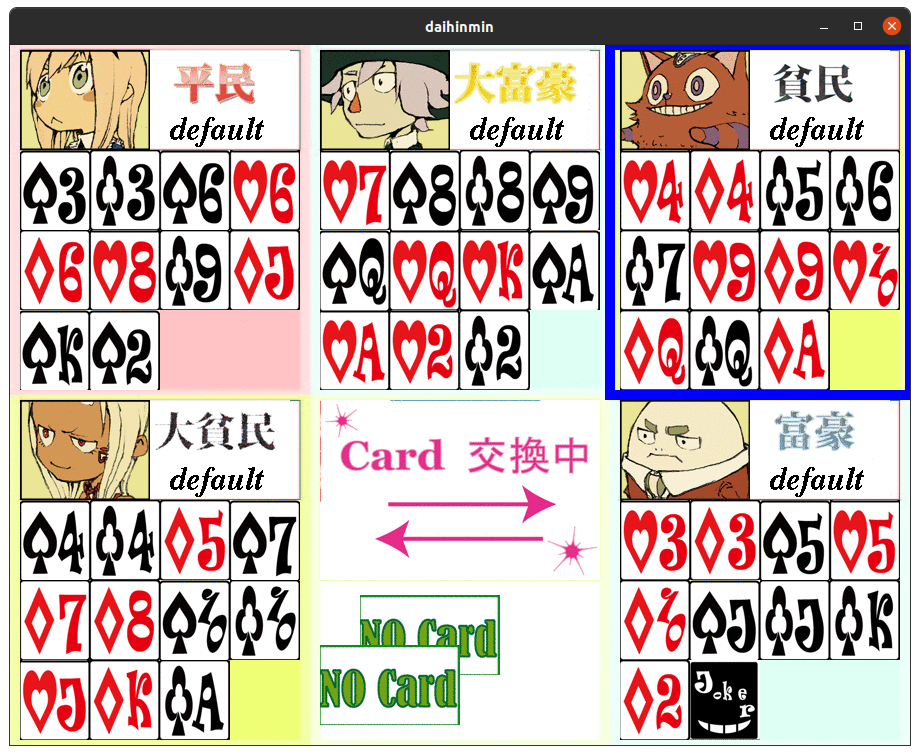
\includegraphics[width=\textwidth]{kadai5/1.png}


\newpage
\section*{課題6(ペア出し機能の実装)}
コンピュータ大貧民教育用クライアントのディレクトリ src にある、select\_cards.c などを改変し、ペア出し機能を実現した。
この課題では、場にカードがない状況で、かつ提出するカードにジョーカーを含まない場合について実装した。
実装が完了したら、大貧民サーバを立ち上げゲームを実行し、ペア出しが行われている様子がわかるスクリーンショットを取得した。
(サーバの実行画面中のクライアントプログラムが Normal と表示されているか、確認した)。\\

\noindent また、実現したペア出し機能について、以下の考察を行った。\\
1。配列をどのように使って処理をしているか。\\
2。該当するソースコードの記述によって何故その機能が実現できているのか。\\

\section*{課題6の実行結果}



\newpage
\begin{thebibliography}{99}
  \bibitem{cite1} 第2回 動的データ構造と再起処理(スタック、二分木), \\URL : \url{https://www.ied.inf.uec.ac.jp/text/laboratory/C/second_week/index02.html}
\end{thebibliography}


\end{document}